\documentclass[12pt]{article}

\usepackage{sbc-template}
\usepackage{graphicx,url}
\usepackage{float}
\usepackage[utf8]{inputenc}
\usepackage[brazil]{babel}
\usepackage[latin1]{inputenc}  

     
\sloppy

\title{Simulated Annealing\\ Uma resolução para Caixeiro Viajante}

\author{César Eduardo de Souza\inst{1},\\ Guilherme Diel\inst{1}}


  \address{Departamento de Ciência da Computação \\ Universidade do Estado de Santa Catarina
  (UDESC) -- Joinville, SC -- Brazil
  \email{\{cesar.souza, guilherme.diel\}@edu.udesc.br}
}

\begin{document} 

\maketitle

     
\begin{resumo} 
  Algoritmos heurísticos se alicerçam em técnicas de busca de solução satisfatória. Um deles é o \textbf{Simulated Annealing}, que se baseia no processo de resfriamento de metais. Este algoritmo é capaz de resolver problemas NP-Hard e NP-Completo, como o problema do \textbf{Caixeiro Viajante}, que consiste em determinar o ciclo de menor custo que percorre um conjunto de cidades, visitando cada uma exatamente uma vez e retornando ao ponto de partida. Neste trabalho, apresentamos uma implementação do \textbf{Simulated Annealing} para resolver o problema do Caixeiro Viajante, com resultados satisfatórios e consistentes, principalmente para instâncias de maior dimensão. Além disso, discutimos possíveis aplicações futuras e comparações com outras abordagens.
\end{resumo}


\section{Introdução}
\label{sec:introducao}
% Contextualização do problema/tarefa e revisão da literatura.
Foi no século XX que se iniciou a busca pela resolução de problemas NP, NP-Hard e NP-Completo usando ferramentas computacionais. 
%
Estas, portanto, foram, em sua maioria, desenvolvidas com base em algoritmos heurísticos — alicerçados em técnicas de busca de solução não necessariamente ótimas, mas sim satisfatórias. — 
%
Sendo assim, alguns destes tornaram-se mais disseminados na literatura científica, como a \textbf{Busca Gulosa}, \textbf{Algoritmo A*}, \textbf{Subida de Encosta} e \textbf{Simulated Annealing}.

O método de \textbf{Simulated Annealing} teve sua lógica concebida a partir do método de anelização de materiais, Metropolis, desenvolvido por Gibbs em 1953.
%
Baseado na fabricação de anéis, este método usa como base o fato de que, quanto mais quente está o material, maior se torna a facilidade de moldá-lo.%
Sob o mesmo ponto de vista, este método consiste em uma sequência de temperaturas decrescentes em que, quanto maior a temperatura atual, mais aleatorizadas são as otimizações geradas pelo algoritmo, sendo que, quando a temperatura chega a um certo ponto, idealiza-se a otimização do resultado conforme decresce a temperatura, até que esta se torne mínima.

Um problema muito conhecido e discutido na literatura, que é capaz de ser resolvido por algoritmos heurísticos, é o problema do \textbf{Caixeiro Viajante} (\textit{Traveling Salesman Problem} - TSP), que consiste em, dado um conjunto de cidades e as distâncias entre cada par de cidades, determinar o ciclo hamiltoniano de custo mínimo que visita cada cidade exatamente uma vez e retorna à cidade de origem.
%
Formalmente, dado um conjunto finito de vértices \( V = \{v_1, v_2, \dots, v_n\} \) e uma função de custo \( c: V \times V \to \mathbb{R}^+ \), o objetivo é encontrar uma permutação \( \pi \in S_n \) que minimize o custo total da rota, ou seja:

\begin{equation}
\min_{\pi \in S_n} \left( c(v_{\pi(1)}, v_{\pi(2)}) + c(v_{\pi(2)}, v_{\pi(3)}) + \dots + c(v_{\pi(n)}, v_{\pi(1)}) \right)
\end{equation}

Ao longo deste relatório, será abordada uma proposta de implementação do \textbf{Simulated Annealing} para resolução do problema do Caixeiro Viajante, um problema NP-Completo que consiste em encontrar o ciclo hamiltoniano de menor custo.

Este relatório está organizado da seguinte maneira: a seção 2 apresenta estratégias utilizadas, descrições, justificativas de escolhas, fórmulas utilizadas e descrições. Em seguida, na seção 3 são abordadas descrições dos experimentos, configurações utilizadas e descrições dos resultados obtidos. Outrossim, na seção 4 expõem-se considerações sobre os resultados obtidos e análises críticas sobre os mesmos. Por fim, na seção 5 mostram-se considerações sobre o trabalho desenvolvido e identificação de direcionamentos futuros na pesquisa.

% Justificativa e motivação.
% Objetivo.
% Organização do texto.

\section{Metodologia de Desenvolvimento}
\label{sec:metodologia_de_desenvolvimento}

O método de \textbf{Simulated Annealing} consiste em:
\begin{enumerate}
  
  \item Para uma temperatura $T_i$, realizar $N$ vezes: \label{passo:1}
  \begin{itemize}
    \item Realizar uma perturbação aleatória no estado atual $\text{estado}_0$, gerando um novo $\text{estado}_i$
    \item Calcular a variação de energia $\Delta E = E(\text{estado}_i) - E(\text{estado}_0)$
    \item Se $\Delta E < 0$ (melhora na energia), aceitar a transição ($\text{estado}_i \rightarrow \text{estado}_0$)
    \item Caso contrário, aceitar a transição com probabilidade P_{\text{accept}}($T_i$)
  \end{itemize}
  
  \item Critério de parada:
  \begin{itemize} \label{passo:2}
    \item Se $T_i \leq T_f$ (temperatura final) ou o sistema atingir convergência (e.g., $\Delta E \approx 0$ por $k$ iterações consecutivas)
    \item Retornar o $\text{estado}_0$ como solução
    \item Caso contrário, reduzir a temperatura ($T_i \leftarrow \alpha T_i$, com $0 < \alpha < 1$) e retornar ao Passo~\ref{passo:1}
  \end{itemize}
  \label{pseudocodigo}
  \caption{Passo a passo do método de \textbf{Simulated Annealing}}
\end{enumerate} 

A aplicação do método de \textbf{Simulated Annealing} para a otimização do problema do Caixeiro Viajante foi realizada por meio da linguagem de programação \textit{Python}, junto com a biblioteca \textit{Numpy}.
%
A Figura \ref{fig:metodologia} retrata o passo a passo de como foi implementado este algoritmo.

A Figura~\ref{fig:metodologia} apresenta as etapas do algoritmo, que foi implementado da seguinte maneira:

\begin{enumerate}
    \item \textbf{Inicialização}:
    \begin{itemize}
        \item Temperatura inicial $T_0 = 1000$
        \item Taxa de resfriamento $\alpha = 0.99$
        \item Temperatura final $T_f = 0.1$
        \item Número de iterações por temperatura $N = 1000$
        \item $SA_{max} = 1$, 5 ou 10 (limite mínimo de temperatura)
    \end{itemize}
    
    \item \textbf{Iteração por temperatura}:
    \begin{enumerate}
        \item Gerar nova solução aleatória (modificando uma variável)
        \item Calcular $\delta E = E_{\text{nova}} - E_{\text{atual}}$
        \item Se $\delta E < 0$, aceitar a nova solução
        \item Caso contrário, aceitar com probabilidade:
        \begin{equation}
            P_{\text{accept}} = \exp\left(-\frac{\Delta E}{T_i}\right)
            \label{eq:probabilidade}
        \end{equation}
    \end{enumerate}
    
    \item \textbf{Resfriamento}:
    \begin{enumerate}
      \item Foram utilizados 3 tipos diferentes de funções de diminuição de temperatura: \textbf{Linear}, \textbf{Exponencial} e \textbf{Logaritmo}
      \item Verificar critério de parada:
        \begin{itemize}
            \item Se $T_i \leq T_{min}$ $\rightarrow$ Parar
            \item Caso contrário $\rightarrow$ Voltar ao passo 2
        \end{itemize}
    \end{enumerate}
\end{enumerate}

\begin{figure}[H]
    \centering
    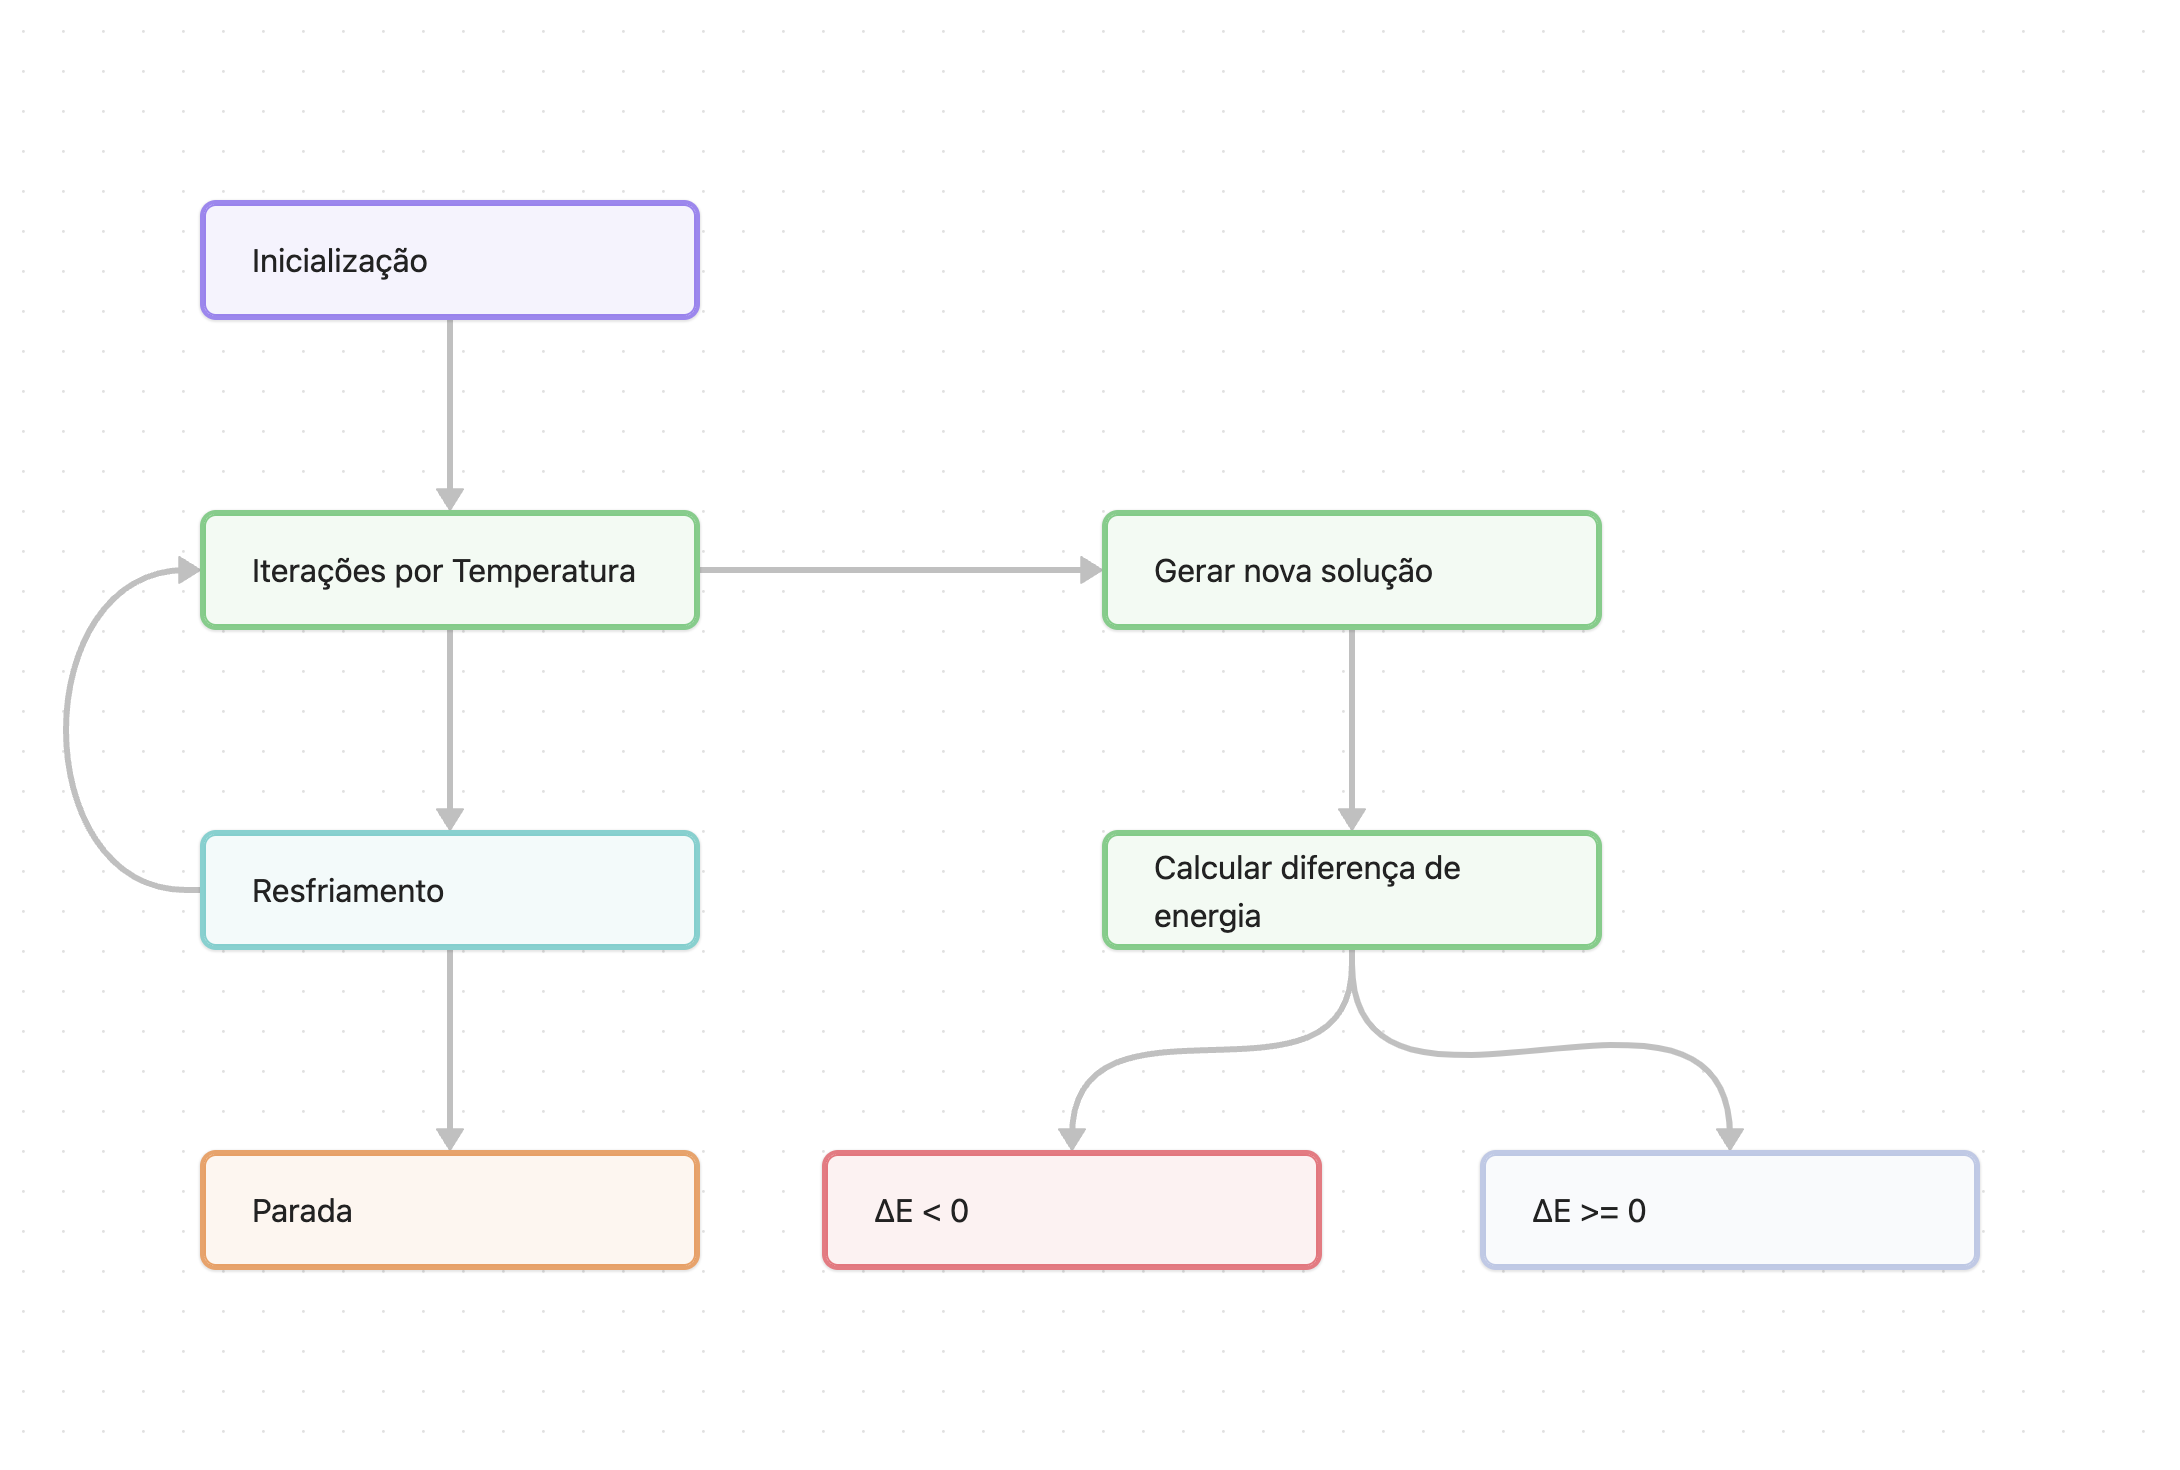
\includegraphics[width=1\textwidth]{imgs/final_diagram.png}
    \caption{Diagrama do algoritmo de \textbf{Simulated Annealing}}
    \label{fig:metodologia}
\end{figure}

% descrições e justificativas das escolhas.
% Fórmulas utilizadas, descrições e justificativas.

\section{Descrição de Experimentos/Simulações e Resultados Obtidos}
\label{sec:descicao_de_experimentos_/_simulacoes_e_resultados_obtidos}

% Descrição dos experimentos
% e configurações utilizadas.
As configurações utilizadas foram: Temperatura inicial = 1.000, Temperatura minima = 0.01. A taxa de resfriamento foi de 3 tipos diferentes: Linear, Exponencial e Logarítmica. 
%
Na linear, a temperatura diminuiu de 1 em 1, enquanto na exponencial diminuiu sempre 95\% da temperatura atual e na logarítmica diminuiu segundo a função: Temperatura atual / (1 + 0.001 * iteração)

% Descrição dos resultados obtidos (Figuras, Tabelas, Gráficos).

Nestas configurações foram obtidos resultados para bases de eil51 e kroA100 como os seguintes gráficos de convergência, com o SA de 1 a 10 nas respectivas figuras \ref{fig:convergencia51} e \ref{fig:convergencia100}.

Conseguimos perceber que todos os gráficos chegaram a energia final parecida, entretanto, quanto maior o $SA_{MAX}$, melhor tende a ser o resultado final.

\begin{figure}[H]
  \centering
  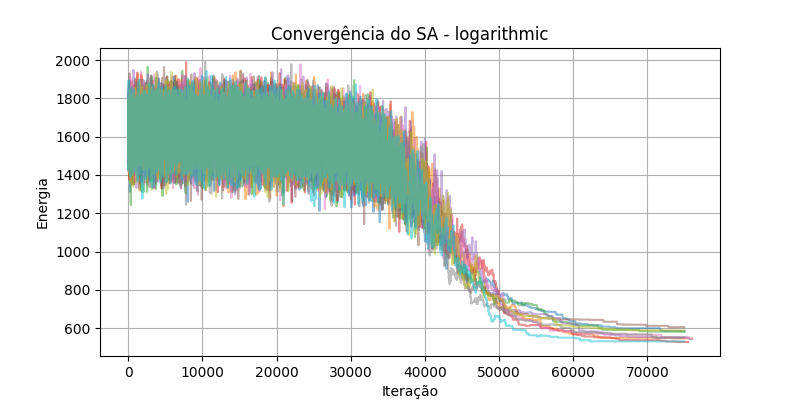
\includegraphics[width=.9\textwidth]{imgs/convergence_51.png}
  \caption{Convergência para eil51}
  \label{fig:convergencia51}
  \end{figure}

\begin{figure}[H]
  \centering
  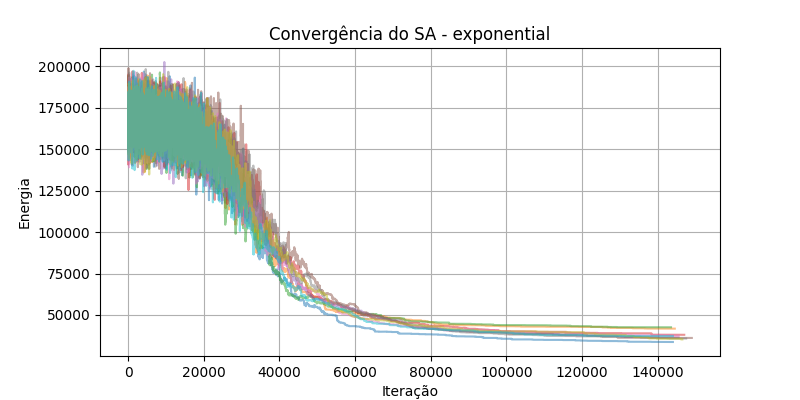
\includegraphics[width=.9\textwidth]{imgs/convergence_100.png}
  \caption{Convergência para kroA100}
  \label{fig:convergencia100}
   \end{figure}

Ademais, foi gerado os boxplots para cada um dos 3 tipos de funções de diminuição de temperatura, com os respectivos resultados obtidos, conforme as figuras \ref{fig:boxplot51} e \ref{fig:boxplot100}.

Aqui é possível perceber que no arquivo com menor quantidade de nós \ref{fig:boxplot51}, o exponencial deu o melhor resultado. 
Porém, no maior arquivo, o resultado \ref{fig:boxplot100} foi o linear que apresentou o melhor resultado.

\begin{figure}[H]
  \centering
  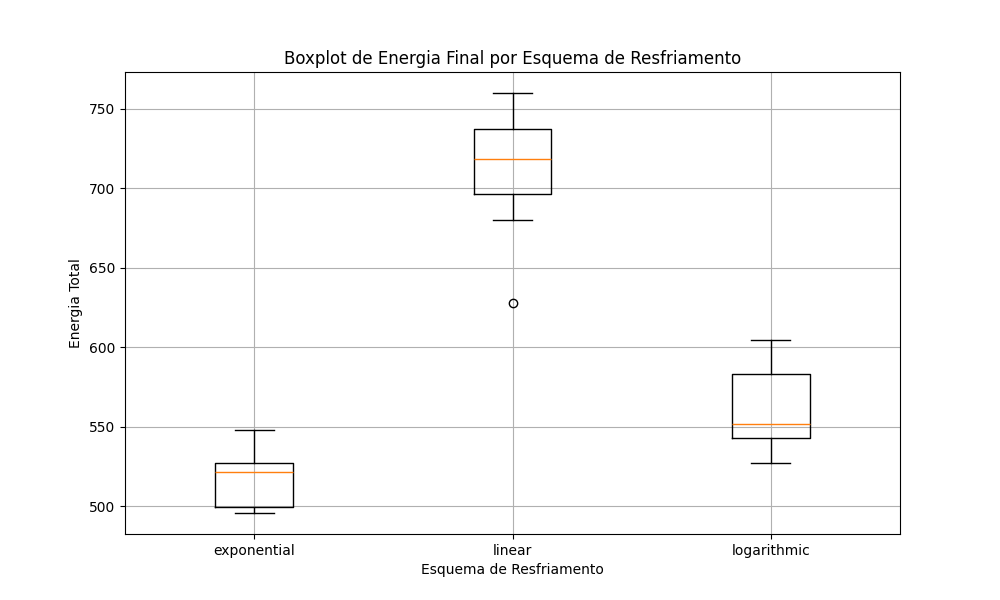
\includegraphics[width=.9\textwidth]{imgs/boxplot_51.png}
  \caption{Boxplots para eil51}
  \label{fig:boxplot51}
\end{figure}

\begin{figure}[H]
  \centering
  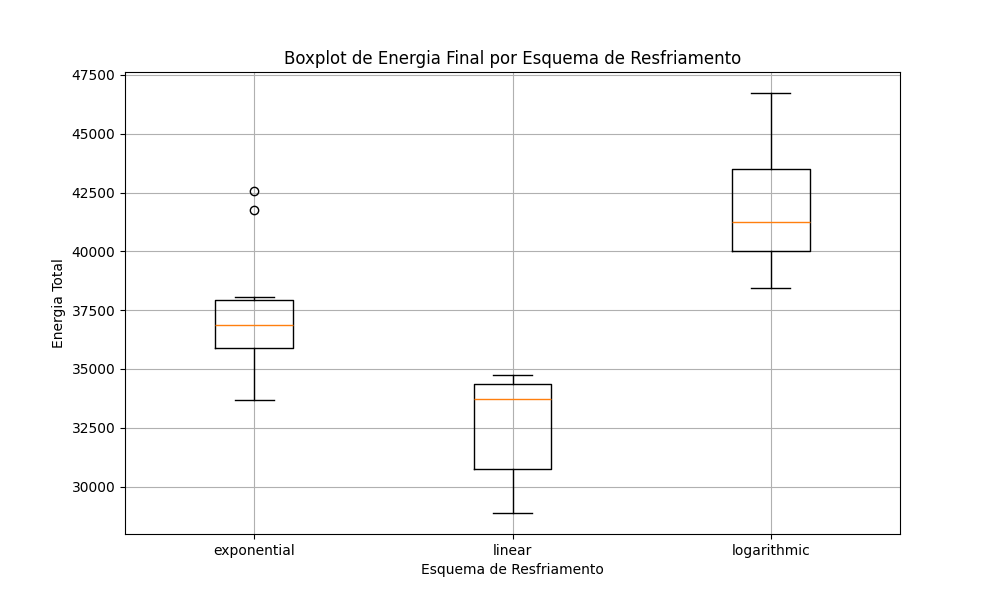
\includegraphics[width=.9\textwidth]{imgs/boxplot_100 copy.png}
  \caption{Boxplots para kroA100}
  \label{fig:boxplot100}
\end{figure}

Além disso, é possível verificar a seguinte tabela com média e desvio padrão de 30 execuções do experimento, apontados pelos consecutivos boxplots.

A tabela confirma o que os gráficos mostraram, de maneira que mostra o exponencial como o melhor resultado para o menor arquivo, enquanto o linear foi o melhor resultado para o maior arquivo.

\begin{table}[H]
\centering
\caption{Média e Desvio Padrão dos Resultados Obtidos}
\begin{tabular}{|c|c|c|c|}
\hline
\textbf{Arquivo} & \textbf{Algoritmo de Resfriamento} & \textbf{Média} & \textbf{Desvio Padrão} \\ \hline
eli51     & EXP     & 517.55      & 17.44 \\ \hline
eli51     & LINEAR  & 712.49      & 36.62 \\ \hline
eli51     & LOG     & 560.58      & 25.29 \\ \hline
kroA100   & EXP     & 37455.66    & 2638.58 \\ \hline
kroA100   & LINEAR  & 32617.12    & 2189.60 \\ \hline
kroA100   & LOG     & 41868.92    & 2443.86 \\ \hline


\end{tabular}
\label{tab:resultados}
\end{table}


Dessa maneira, é possível obter uma visão aprofundada da execução do algoritmo, discutida na seção a seguir.

\section{Análise dos resultados obtidos.}
\label{sec:analise_dos_resultados_obtidos}

A análise dos resultados obtidos permite verificar a influência significativa da estratégia de resfriamento na qualidade das soluções encontradas pelo algoritmo de \textbf{Simulated Annealing} para o problema do Caixeiro Viajante. Os dados apresentados demonstram que, embora todas as abordagens de resfriamento tenham convergido para soluções de energia final semelhante, a taxa de resfriamento e a quantidade de iterações (\( SA_{MAX} \)) impactaram diretamente a qualidade da solução final.

Observa-se que, para a instância \textit{eil51}, de menor dimensão, a estratégia de resfriamento exponencial apresentou desempenho superior, obtendo a menor média de custo e o menor desvio padrão. Este comportamento pode ser atribuído ao fato de que, em instâncias menores, uma redução mais rápida da temperatura favorece a exploração eficiente do espaço de soluções, evitando a estagnação em mínimos locais sem comprometer a convergência.

Em contraste, para a instância \textit{kroA100}, de maior dimensão, o resfriamento linear demonstrou desempenho superior. A diminuição gradual e uniforme da temperatura parece ter permitido uma exploração mais robusta do espaço de soluções, resultando em soluções de menor custo médio e menor variabilidade em relação às demais estratégias. Esse comportamento sugere que, em instâncias mais complexas, uma taxa de resfriamento mais conservadora contribui para um equilíbrio mais eficaz entre exploração e intensificação.

Adicionalmente, constata-se que, independentemente da estratégia de resfriamento, o aumento de \( SA_{MAX} \) resultou, de forma consistente, em melhores soluções finais, evidenciando a relevância da quantidade de iterações no desempenho do algoritmo.

Portanto, conclui-se que a escolha da estratégia de resfriamento deve considerar a dimensão e a complexidade da instância do problema, sendo o resfriamento exponencial mais adequado para instâncias menores e o resfriamento linear mais indicado para instâncias maiores. Esta constatação destaca a necessidade de parametrização criteriosa para maximizar a eficiência do \textbf{Simulated Annealing} na resolução do problema do Caixeiro Viajante.

\section{Conclusões e Trabalhos Futuros}
\label{sec:conclusoes_e_trabalhos_futuros}

Neste trabalho, foi apresentada uma implementação do algoritmo de \textbf{Simulated Annealing} aplicado à resolução do problema do Caixeiro Viajante, avaliando o impacto de diferentes estratégias de resfriamento sobre a qualidade das soluções obtidas. As análises realizadas demonstraram que a escolha da função de resfriamento exerce influência relevante no desempenho do algoritmo, sendo que o resfriamento exponencial apresentou melhores resultados em instâncias de menor dimensão, enquanto o resfriamento linear se mostrou mais eficaz em instâncias de maior complexidade.

Além disso, verificou-se que o aumento do número de iterações contribui consistentemente para a obtenção de soluções mais próximas do ótimo, reforçando a importância de uma parametrização adequada conforme a instância do problema.

Como trabalhos futuros, propõe-se a realização de experimentos adicionais utilizando outras instâncias clássicas do problema do Caixeiro Viajante, de diferentes tamanhos e características, a fim de validar a generalização dos resultados obtidos. Ademais, sugere-se a investigação de estratégias híbridas, combinando \textbf{Simulated Annealing} com outros métodos heurísticos ou metaheurísticos, como algoritmos genéticos ou busca tabu, visando potencializar a eficiência e a robustez da abordagem.

Outra linha de pesquisa promissora consiste na adaptação dinâmica da taxa de resfriamento durante a execução do algoritmo, com base em métricas de desempenho em tempo de execução, de forma a automatizar a escolha da estratégia mais adequada conforme o comportamento da busca.

Dessa forma, espera-se que os avanços futuros ampliem a aplicabilidade e a eficácia do \textbf{Simulated Annealing} na resolução de problemas de otimização combinatória, em especial o problema do Caixeiro Viajante.


\bibliographystyle{sbc}
\bibliography{sbc-template}

\end{document}
